\documentclass[12pt]{article}
\usepackage[utf8]{inputenc} % Pacote para acentuação gráfica
%\usepackage[T1]{fontenc}
\usepackage[brazil]{babel} % nomes das estruturas em pt-br
%\usepackage{hyperref}
\usepackage{indentfirst} % indenta primeiro paragráfo após título
\usepackage{setspace} % pacote para alterar espaçamento entre linhas
%\setlength{\parindent}{1cm} % define o tamanho da indentação
%\setlength{\parskip}{0.3cm} % define o espaçamento vertical entre parágrafos
\usepackage[top = 2cm, left = 2cm, bottom = 2cm, right = 2cm]{geometry} % define as margens do documento
\usepackage{fancyhdr} % pacote para numeração de páginas
\usepackage{hyperref}
\usepackage[table,xcdraw]{xcolor} % tabela colorida
\usepackage{float} % força posição de tabelas e figuras
\usepackage{graphicx}

\usepackage{xcolor}
% Definindo novas cores
\definecolor{verde}{rgb}{0.25,0.5,0.35}
\definecolor{jpurple}{rgb}{0.5,0,0.35}
% Configurando layout para mostrar codigos Java
\usepackage{listings}
\lstset{
	language=Java,
	basicstyle=\ttfamily\small,
	keywordstyle=\color{jpurple}\bfseries,
	stringstyle=\color{red},
	commentstyle=\color{verde},
	morecomment=[s][\color{blue}]{/**}{*/},
	extendedchars=true,
	showspaces=false,
	showstringspaces=false,
	numbers=left,
	numberstyle=\tiny,
	breaklines=true,
	backgroundcolor=\color{cyan!10},
	breakautoindent=true,
	captionpos=b,
	xleftmargin=0pt,
	tabsize=4
}
\pagestyle{empty}

\begin{document}
	
\title{\textbf{{\Huge 1Z0-808 - Notas de Estudo}}} % Título
\author{\textbf{{\Large Ricardo Alvarenga}}} % Autor
\date{\textbf{{\Large 2024}}} % Data
\maketitle % Criar
\thispagestyle{empty} % remove número da página
\newpage

\section*{Como Tirar a Certificação Entre 3 e 6 Meses de Estudo}

Referência: \url{https://www.youtube.com/watch?v=t-7GVhoM0bY&t=889s&ab_channel=Jos%C3%A9Castilho-DesenvolvedorDisputado}

\subsection*{Por Quê Tirar a Certificação Java}

\begin{itemize}
	\item Poucos profissionais são certificados;
	\item Gera reconhecimento;
	\item São duas certificações, a primeira \textbf{Java SE Programmer I exam (1Z0-808)}. A segunda querer a primeira e possui várias áreas distintas;
\end{itemize}

\subsection*{Método Sugerido}

\begin{itemize}
	\item Aprender a linguagem, não começar por livro preparatório. Usar livros básicos primeiro;
	\item Estudar com data definida;
	\item "Comer" um livro de certificação;
	\item Usar várias metodologias. Alguns assuntos são assimilados melhor com leitura, outros com vídeos, outros \textit{codando} e vendo funcionar;
	\item Fazer muitos simulados. Simular provas até conseguir notas altas em várias provas simuladas;
	\item Aprender com os erros e acertos dos simulados;
	\item Repetir o ciclo de fazer simulados e analisar erros e acertos, várias vezes;
\end{itemize}

\newpage

\setcounter{page}{1} % reset contador de página
\pagenumbering{Roman}
\tableofcontents % cria sumário
\pagestyle{fancy}
\fancyfoot[C]{\thepage} % Adiciona o número da página no centro do rodapé
\newpage

\listoffigures % lista de figuras
\newpage

\setcounter{page}{1} % reset contador de página
\pagenumbering{arabic}
\pagestyle{fancy}
\fancyfoot[C]{\thepage}


\section{Java Basics}
\subsection{Define the scope of variables}

O escopo é o que determina em que pontos do código uma variável pode ser usada.

\subsubsection{Variáveis locais}

Variáveis locais são declaradas dentro de métodos ou construtores. O ciclo de vida de uma variável local vai do ponto onde ela foi declarada até o fim do daquele bloco.

Quando a execução sai do escopo a variável não pode mais ser usada e seu valor é perdido. A qualquer momento o JVM pode realocar a memória ocupada por ela.

Bloco é um trecho de código entre chaves \textbf{\textit{{}}}. Pode ser um método, um construtor, o corpo de um \textbf{\textit{if}}, de um \textbf{\textit{for}} etc.

Analise o código abaixo e identifique os escopos de \textbf{\textit{x}} e \textbf{\textit{y}}:

\begin{lstlisting}
public void m1() { // inicio do bloco do metodo
	int x = 10; // variavel local do metodo
	
	if (x >= 10) { // inicio do bloco do if
		int y = 50; // variavel local do if
		System.out.print(y);
	} // fim do bloco do if
} // fim do bloco do metodo
\end{lstlisting}



Tome cuidado especial com loops \textbf{\textit{for}}. As variáveis declaradas na área de inicialização do loop só podem ser usadas no corpo do loop:

\begin{lstlisting}
for (int i = 0, j = 0; i < 10; i++) j++;

System.out.println(j); // erro, ja nao esta mais no escopo
\end{lstlisting}

Parâmetros de métodos também podem ser considerados variáveis locais ao método, ou seja, só podem ser usados dentro do método onde foram declarados:

\begin{lstlisting}
class Teste {
	
	public void m1(String bla) {
		System.out.print(bla);
	}
	
	public void m2() {
		// erro de compilacao pois bla nao existe neste
		// escopo
		System.out.println(bla);
	}
}
\end{lstlisting}

Os parâmetros podem ser primitivos ou objetos. Um método pode ter até 255 parâmetros. Essas variáveis fazem parte do escopo do bloco do método inteiro e são definidas na declaração do método.
\pagebreak

\begin{lstlisting}
float findMilesPerHour(float milesTraveled, float hoursTraveled){
	//o metodo contem dois parametros
	return milesTraveled / hoursTraveled;
}
\end{lstlisting}

\subsubsection{Variáveis de instância}

Variáveis de instância ou variáveis de objeto são os atributos dos objetos. São declaradas dentro da classe, mas fora de qualquer método ou construtor. Fazem parte do escopo da classe. Podem ser acessadas por qualquer membro da classe e ficam em escopo enquanto o objeto existir:

\begin{lstlisting}
class Pessoa {
	// variavel de instancia ou variavel de objeto
	String nome;
	
	public void setNome(String n) {
		// acessando a variavel de instancia no metodo
		this.nome = n;
	}
}
\end{lstlisting}

\subsubsection{Variáveis estáticas (class variables)}

Podemos declarar variáveis que são compartilhadas por todas as instâncias de uma classe usando a palavra chave \textbf{\textit{static}}. Essas variáveis estão no escopo da classe, e lá ficarão enquanto a classe estiver carregada na memória (enquanto o programa estiver rodando, na grande maioria dos casos).

\begin{lstlisting}
class Pessoa {
	static int id = 1;
}
	
class Teste {
	public static void main(String[] args) {
		Pessoa p = new Pessoa();
		System.out.println(p.id); // acessando pelo objeto. id = 1
		System.out.println(Pessoa.id); // acessando direto pela classe.
		                               // id = 1
		p.id ++; // soma 1
		System.out.println(Pessoa.id); // id = 2
		p.id ++;
		Pessoa pp = new Pessoa(); 
		p.id ++;
		System.out.println(pp.id); // id = 4
		System.out.println(Pessoa.id); // id = 4
	}
}
\end{lstlisting}

No caso de variáveis \textbf{\textit{static}}, não precisamos ter uma referência para usá-las e podemos acessá-las diretamente a partir da classe, desde que respeitando as regras de visibilidade da variável.

\subsubsection{Variáveis com o mesmo nome}

Não é possível declarar duas variáveis no mesmo escopo com o mesmo nome:

\begin{lstlisting}
public void bla() {
	int a = 0;
	int a = 10;// erro
}
\end{lstlisting}

Mas, eventualmente, podemos ter variáveis em escopos diferentes que podem ser declaradas com o mesmo nome. Em casos em que possa haver ambiguidade na hora de declará-las, o próprio compilador irá emitir um erro evitando a confusão.

Por exemplo, não podemos declarar variáveis de classe e de instância com o mesmo nome:

\begin{lstlisting}
class Bla {
	static int a;
	int a; // erro de compilacao,
}
...
System.out.println(new Bla().a); // qual variavel estamos acessando?
\end{lstlisting}

Também não podemos declarar variáveis locais com o mesmo nome de parâmetros:

\begin{lstlisting}
public void metodo(String par) {
	int par = 0; // erro de compilacao
	
	System.out.println(par); // qual?
}
\end{lstlisting}

Apesar de parecer estranho, é permitido declarar variáveis locais ou parâmetros com o mesmo nome de variáveis de instância ou de classe. Essa técnica é chamada de \textit{shadowing}. Nesses casos, é possível resolver a ambiguidade: para variáveis de classe, podemos referenciar pela própria classe; para variáveis de instância, usamos a palavra chave \textbf{\textit{this}}:

\begin{lstlisting}
class Pessoa {
	
	static int x = 0;
	int y = 0;
	
	public static void setX(int x) {
		// Usando a referencia da classe
		Pessoa.x = x;
	}
	
	public void setY(int y) {
		// usando o this
		this.y = y;
	}
}
\end{lstlisting}
\pagebreak
Quando não usamos o \textbf{\textit{this}} ou o nome da classe para usar a variável, o compilador sempre utilizará a variável de menor escopo:

\begin{lstlisting}
class X {
	int a = 10;
	
	public void metodo() {
		int a = 20; // shadowing
		System.out.println(a); // imprime 20
	}
}
\end{lstlisting}

\subsubsection{Difference Between \textit{Life} and \textit{Scope} For Local Variables}

\textbf{\textit{Life:}} A local variable is \textit{alive} as long as its Stack frame is on the Stack. In other words, \textit{until the method completes}.

\textbf{\textit{Scope:}} A local variable is in \textit{scope} only within the method in which the variable was declared. When its own method calls another, the variable is alive, but not in scope until its method resumes. \textbf{You can use a variable only when it is in scope}.


% Please add the following required packages to your document preamble:
% \usepackage[table,xcdraw]{xcolor}
% Beamer presentation requires \usepackage{colortbl} instead of \usepackage[table,xcdraw]{xcolor}
\begin{table}[H]
	\begin{tabular}{|ll|}
		\hline
		\multicolumn{2}{|c|}{\cellcolor[HTML]{34FF34}\textit{\textbf{Cenário e Solução}}}                                        \\ \hline
		\multicolumn{1}{|l|}{Variável mais adequada para um contador em um laço?}                        & Variável local        \\ \hline
		\multicolumn{1}{|l|}{Variável deve ser usada para armazenar informações sobre um objeto?}        & Variável de instância \\ \hline
		\multicolumn{1}{|l|}{Que variável deve ser usada para a passagem de informações para um método?} & Parâmetro de método   \\ \hline
	\end{tabular}
\end{table}

\subsection{Define the structure of a Java class}

Nesta seção, iremos entender a estrutura de um arquivo java, onde inserir as declarações de pacotes e imports e como declarar classes e interfaces.

Para entender a estrutura de uma classe, vamos ver o arquivo \textbf{\textit{Pessoa.java}}:

\begin{lstlisting}
// Declaracao de pacote
package br.com.alvarenga.certificacao;
	
// imports
import java.util.Date;
	
// Declaracao da classe
class Pessoa {
	// conteudo da classe
}
\end{lstlisting}

\subsubsection{Pacotes}

Pacotes servem para separar e organizar as diversas classes que temos em nossos sistemas. Todas as classes pertencem a um pacote, sendo que, caso o pacote não seja explicitamente declarado, a classe fará parte do que chamamos de pacote padrão, ou \textbf{\textit{default package}}. Todas as classes no \textbf{\textit{default package}} se enxergam e podem ser utilizadas entre si. Classes no pacote \textbf{\textit{default}} \textbf{\textit{NÃO}} \textbf{podem ser importadas para uso em outros pacotes}.

\begin{lstlisting}
// Uma classe no pacote padrao
class Pessoa {
	//...
}
\end{lstlisting}

Para definir qual o pacote a que a classe pertence, usamos a palavra-chave \textbf{\textit{package}}, seguida do nome do pacote. \textbf{Só pode existir um único \textbf{\textit{package}} definido por arquivo, e ele deve ser a primeira instrução do arquivo.} Após a definição do \textbf{\textit{package}}, devemos finalizar a instrução com um \textbf{\textit{;}}. \textbf{Podem existir comentários antes da definição de um pacote}:

\begin{lstlisting}
// declaracao do pacote
package br.com.alvarenga.certificacao;
	
class Pessoa {
	//...
}
\end{lstlisting}

\textbf{\textit{Package}} deve ser a primeira instrução de código que temos declarada em nosso arquivo. Comentários não são considerados parte do código, portanto, podem existir em qualquer lugar do arquivo Java sem restrições.

Formas para inserir comentários:

\begin{lstlisting}
// comentario de linha

/*
comentario de
multiplas linhas
*/
class /* comentario no meio da linha */ Pessoa {
	
	/**
	*  JavaDoc, repare que a primeira linha do comentario tem
	*  2 asteriscos
	*/
	public void metodo() {
	}
}
\end{lstlisting}

\subsubsection{Classe}

Uma classe é a forma no Java onde definimos os atributos e comportamentos de um objeto. A declaração de uma classe pode ser bem simples, apenas a palavra \textbf{\textit{class}} seguida do nome e de \textbf{\textit{\{\}}}:

\begin{lstlisting}
class Pessoa {}
\end{lstlisting}

Existem outros modificadores que podem ser usados na definição de uma classe, mas veremos essas outras opções mais à frente, onde discutiremos esses modificadores com mais detalhes.

Vale lembrar que java é case \textit{sensitive} e \textbf{\textit{Class}} é o nome de uma classe e não podemos usá-lo para definir uma nova classe.
\pagebreak

Dentro de uma classe, podemos ter variáveis, métodos e construtores. Essas estruturas são chamadas de \textbf{membros da classe}.:

\begin{lstlisting}
class Pessoa {
	
	String nome;
	String sobrenome;
	
	Pessoa(String nome, String sobrenome) {
		this.nome = nome;
		this.sobrenome = sobrenome;
	}
	
	public String getNomeCompleto() {
		return this.nome + this.sobrenome;
	}
}	
\end{lstlisting}

% TODO: \usepackage{graphicx} required
\begin{figure}[H]
	\centering
	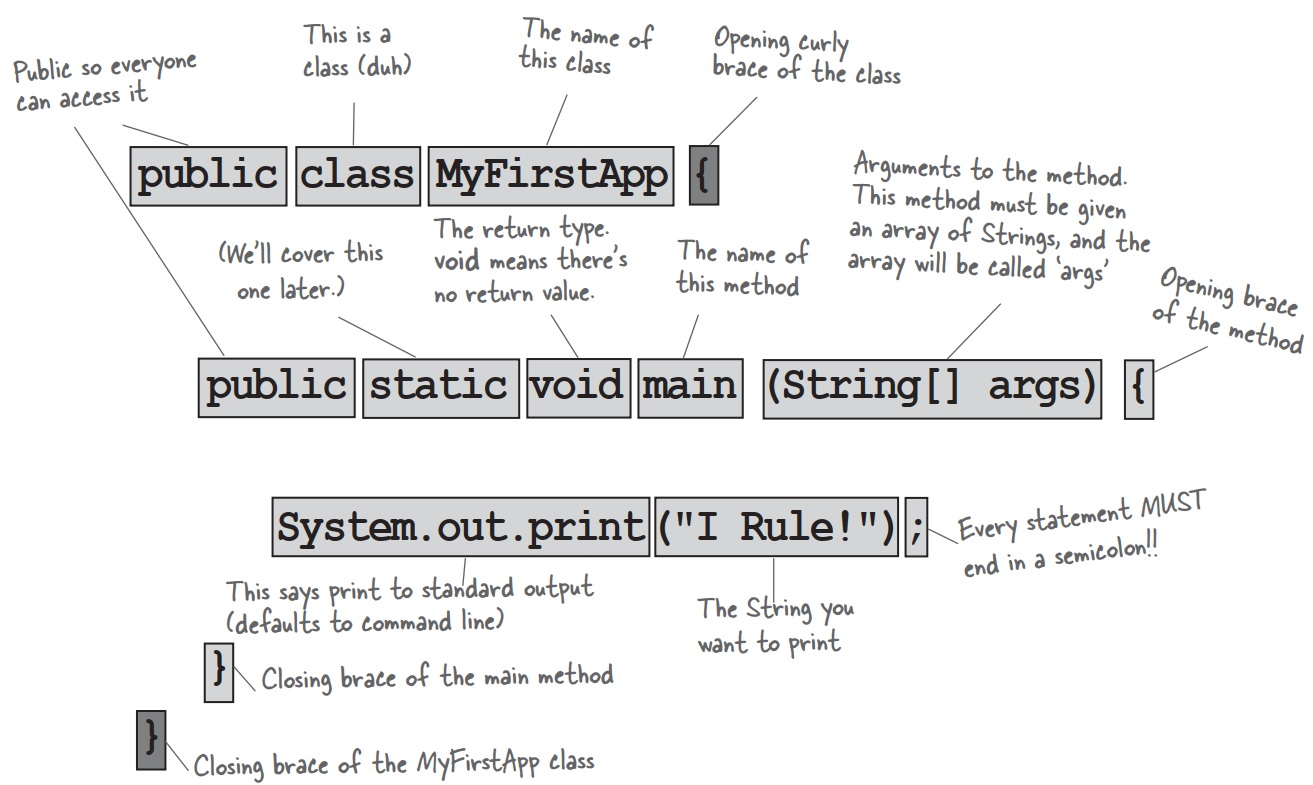
\includegraphics[width=1\linewidth]{figuras/class}
	\caption[Anatomy of a class]{Anatomy of a class}
	\label{fig:class}
\end{figure}

In Java, everything goes in a class. You’ll type your source code file (with a \textit{.java} extension), then compile it into a new class file (with a \textit{.class} extension). When you run your program, you’re really running a class.


\subsubsection{Variáveis}

No exemplo da classe Pessoa definida anteriormente, \textit{nome} e \textit{sobrenome} são \textbf{variáveis}. A declaração de variáveis: \textit{tipo} \textit{\underline{nome\_da\_variável;}}.

Essas são variáveis de instância, pois existe uma cópia delas para cada objeto \textit{Pessoa} criado. Cada cópia guarda o estado de uma certa instância desses objetos.

Há variáveis que não guardam valores ou referências para uma determinada instância, mas sim um valor compartilhado por todas as instâncias de objetos. Essas são variáveis estáticas, definidas com a palavra-chave \textbf{\textit{static}}.

\subsubsection{Métodos}

Na declaração de métodos precisamos do tipo do retorno, seguido do nome do método e seguido de parênteses, sendo que pode ou não haver parâmetros de entrada desse método. Cada parâmetro é uma declaração de variável em si. Essa linha do método, onde está definido o retorno, o nome e os parâmetros é onde temos a assinatura do método. \textbf{\textit{A assinatura de um método inclui somente o nome do método e os tipos dos parâmetros}}. Métodos também podem ser \textbf{\textit{static}}.

\subsubsection{Construtores}

\textbf{Uma classe pode possuir zero ou vários construtores}. A classe \textit{Pessoa} possui um construtor que recebe como parâmetros o nome e o sobrenome da pessoa. A principal diferença entre a declaração de um método e um construtor é que \textbf{um construtor não tem retorno e possui o mesmo nome da classe}.

\subsubsection{Métodos com o mesmo nome da classe}

Note que um construtor pode ter um \textbf{\textit{return}} vazio:

\begin{lstlisting}
class X {
	int j = -100;
	
	X(int i) {
		if (i > 1)
		return;
		j = i;
	}
}
\end{lstlisting}

Caso o valor seja maior que \textbf{\textit{1}}, o valor de \textbf{\textit{j}} será \textbf{\textit{-100}}, caso contrário, será o mesmo valor de \textbf{\textit{i}}.

\subsubsection{Interfaces}

Para definir uma interface usamos a palavra reservada \textbf{\textit{interface}}:

\begin{lstlisting}
interface Autenticavel {
	
	final int TAMANHO_SENHA = 8;
	
	void autentica(String login, String senha);
}
\end{lstlisting}

Em uma interface, devemos apenas definir a assinatura do método, sem a sua implementação. Além da assinatura de métodos, também é possível declarar constantes em interfaces.

\subsubsection{Múltiplas estruturas em um arquivo}

Em java, é possível definir mais de uma classe/interface em um mesmo arquivo java, embora devamos seguir algumas regras:

\begin{itemize}
	\item Podem ser definidos em qualquer ordem;
	\item Se existir alguma classe/interface pública, o nome do arquivo deve ser o mesmo dessa classe/interface;
	\item Só pode existir uma classe/interface pública por arquivo;
	\item Se não houver nenhuma classe/interface pública, o arquivo pode ter qualquer nome.
\end{itemize}

\begin{lstlisting}
// arquivo1.java
interface Bar {}

class Foo {}
\end{lstlisting}


\begin{lstlisting}
// Foo.java
public class Foo {}

interface X {}
\end{lstlisting}

\subsubsection{Pacotes e imports em arquivos com múltiplas estruturas}

As regras de pacotes e \textbf{\textit{imports}} valem também para arquivos com múltiplas estruturas definidas. Caso exista a definição de um pacote, ela vale para todas as classes/interfaces definidas nesse arquivo, e o mesmo vale para \textbf{\textit{imports}}.

\subsubsection{Convenções de nomenclatura}

\begin{figure}[H]
	\centering
	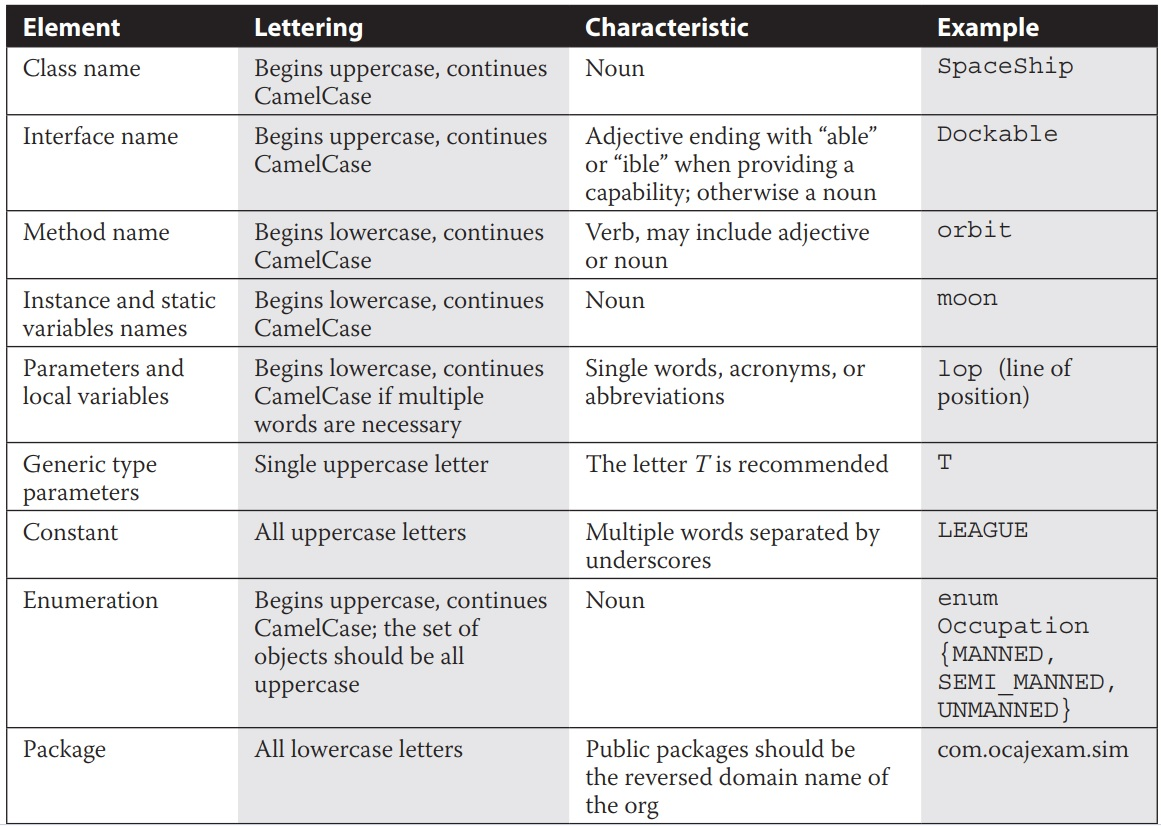
\includegraphics[width=1\linewidth]{figuras/nomenclatura}
	\caption[Nomenclatura Java]{Nomenclatura Java}
	\label{fig:nomenclatura}
\end{figure}

\begin{figure}[H]
	\centering
	\includegraphics[width=1\linewidth]{figuras/símbolos_e_separadores}
	\caption[Símbolos e separadores]{Símbolos e separadores}
	\label{fig:simboloseseparadores}
\end{figure}


\subsection{Create executable Java applications with a main method; run a Java program from the command line; produce console output}

\begin{itemize}
	\item Compilar \textit{javac \textbf{nome\_arquivo.java}}
	\item Executar \textit{java \textbf{nome\_pacote.nome\_classe}}
	\item Método \textit{\textbf{main()}} deve ser \textit{\textbf{public static void}}
\end{itemize}

Uma classe executável é uma classe que possui um método inicial para a execução do programa - o método \textit{main()}, que será chamado pela JVM. Classes sem o método \textit{main()} não são classes executáveis e não podem ser usadas como ponto inicial da aplicação.

\subsubsection{Método \textit{main()}}

Rregras para ser executado pela JVM:
\begin{itemize}
	\item Ser público (\textit{public});
	\item Ser estático (\textit{static});
	\item Não ter retorno (\textit{void});
	\item Ter o nome \textit{main};
	\item Receber como parâmetro um \textit{array} ou \textit{varargs} de \textit{String} (\textit{String[] ou String...}).
\end{itemize}

Exemplos:

\begin{lstlisting}
	//Parametro como array
	public static void main (String[] args) {}
	
	//Parametro como varargs
	public static void main (String... args) {}
	
	//A ordem dos modificadores nao importa
	static public void main(String[] args) {}
	
	//O nome do parametro nao importa
	public static void main (String... argumentos){}
	
	//Tambem e uma definicao valida de array
	public static void main (String args[]) {}
\end{lstlisting}

\subsubsection{Executando uma classe pela linha de comando}

Para executar uma classe com \textit{main()} pela linha de comando, devemos compilar o arquivo com o comando \textit{javac} e executar a classe com o comando \textit{java}. Exemplo com arquivo \textit{HelloWorld.java}:

\begin{lstlisting}
	$ javac HelloWorld.java
	$
	$ java HelloWorld
	Hello World!
\end{lstlisting}

\subsubsection{Passando parâmetros pela linha de comando}

\begin{lstlisting}
public class HelloWorld{
	public static void main(String[] args) {
		//Lendo o valor da primeira posicao do array args
		System.out.println("Hello " + args[0] + "!");
	}
}	
\end{lstlisting}

Informando o parâmetro:

\begin{lstlisting}
java HelloWorld Mario
Hello Mario!
\end{lstlisting}

Os parâmetros devem ser separados por espaço. Cada parâmetro informado será armazenado em uma posição do array, na mesma ordem em que foi informado.

\subsubsection{Compilação e execução}

Para criar um programa java, é preciso escrever um código-fonte e, através de um compilador, gerar o executável (bytecode). O compilador do JDK (Java Development Kit) é o \textit{javac}. Para a prova de certificação, devemos conhecer o comportamento desse compilador.

A execução do bytecode é feita pela JVM (Java Virtual Machine). O comando java invoca a máquina virtual para executar um programa java. Ao baixarmos o Java, podemos escolher baixar o JDK, que já vem com o JRE, ou somente o JRE (Java Runtime Environment), que inclui a Virtual Machine.

Algumas questões da prova abordam aspectos fundamentais do processo de compilação e de execução. É necessário saber como os comandos \textit{javac} e o \textit{java} procuram os arquivos.

\subsubsection{javac}

Arquivo \textit{Prova.java} dentro do diretório do projeto:

\begin{lstlisting}
class Prova {
	double tempo;
}
\end{lstlisting}

\begin{lstlisting}
$ javac Prova.java
\end{lstlisting}

O bytecode da classe \textit{Prova} gerado na compilação é colocado no arquivo \textit{Prova.class} dentro do diretório de trabalho, projeto:

\begin{figure}[H]
	\centering
	
\includegraphics[width=0.7\linewidth]{figuras/estrutura1}
	\caption[Pasta de trabalho]{Pasta de trabalho}
	\label{fig:estrutura1}
\end{figure}


Vejamos qual é o comportamento do \textit{javac} com a utilização de pacotes. Colocamos o arquivo \textit{Prova.java} no diretório \textit{certificacao}:

\begin{lstlisting}
package certificacao;
class Prova {
	double tempo;
}
\end{lstlisting}

\begin{lstlisting}
[certificacao]$ javac certificacao/Prova.java
\end{lstlisting}

Nesse exemplo, o arquivo \textit{Prova.class} é colocado no diretório certificacao.

\begin{figure}[H]
	\centering
	
\includegraphics[width=0.7\linewidth]{figuras/estrutura2}
	\caption[Pasta de trabalho com \textit{package}]{Pasta de trabalho com \textit{package}}
	\label{fig:estrutura2}
\end{figure}

\subsubsection{Escolhendo a versão do Java na hora de compilar}

Na compilação, é possível definir em que versão do Java o código-fonte foi escrito. Isso é feito com a opção \textit{-source} do comando \textit{javac}. (\textit{javac MinhaClasse.java -source 1.3}).

\subsubsection{java}

Como exemplo do comando \textit{java}, criando o arquivo \textit{Teste.java} no mesmo diretório, no mesmo pacote:

\begin{lstlisting}
package certificacao;
class Teste {
	public static void main(String[] args) {
		Prova p = new Prova();
		p.tempo = 210;
		System.out.println(p.tempo);
	}
}
\end{lstlisting}

\begin{lstlisting}
$ javac certificacao/Teste.java
$ java certificacao.Teste
\end{lstlisting}

\begin{lstlisting}
210.0
\end{lstlisting}

\begin{figure}[H]
	\centering
	
\includegraphics[width=0.7\linewidth]{figuras/estrutura3}
	\caption[Pasta de trabalho com \textit{package} e várias classes]{Pasta de trabalho com \textit{package} e várias classes}
	\label{fig:estrutura3}
\end{figure}

Somente o arquivo \textit{Teste.java} foi passado para o compilador. Nesse arquivo, a classe \textit{Teste} utiliza a classe \textit{Prova} que se encontra em outro arquivo, \textit{Prova.java}. Dessa forma, o compilador vai compilar automaticamente o arquivo \textit{Prova.java} se necessário.

Para executar, é preciso passar o nome completo da classe desejada para a máquina virtual. O sufixo \textit{.class} não faz parte do nome da classe, então ele não aparece na invocação da máquina virtual pelo comando \textit{java}.

\subsubsection{Propriedades na linha de comando}

A prova ainda cobra conhecimentos sobre como executar um programa java passando parâmetros ou propriedades para a JVM e essas propriedades são identificadas pelo \textit{-D} antes delas. Este \textit{-D} não faz parte da chave.

\begin{lstlisting}
java -Dchave1=abc -Dchave2=def Foo xpto bar
\end{lstlisting}

\textbf{\textit{chave1=abc}} e \textbf{\textit{chave2=def}} são parâmetros/propriedades e \textbf{\textit{xpto}} e \textbf{\textit{bar}} são argumentos recebidos pelo método \textbf{\textit{main}}.

\subsubsection{Classpath}

Para compilar ou para executar, é necessário que os comandos \textit{javac} e \textit{java} possam encontrar as classes referenciadas pela aplicação java.

A prova de certificação exige o conhecimento do algoritmo de busca das classes. As classes feitas pelo programador são encontradas através do \textit{classpath} (caminho das classes).

O \textit{classpath} é formado por diretórios, jars e zips que contenham as classes e pacotes da nossa aplicação. Por padrão, o \textit{classpath} está configurado para o diretório corrente (\textit{\textbf{.}}).

\subsubsection{Configurando o classpath}

Há duas maneiras de configurar o classpath:

\textbf{1}) Configurando a variável de ambiente \textit{CLASSPATH} no sistema operacional.

Basta seguir as opções do SO em questão e definir a variável. \textbf{Isso é considerado uma má prática no dia a dia} porque é um \textit{classpath} global, que vai valer para qualquer programa java executado na máquina.

\textbf{2}) Com as opções \textit{-cp} ou \textit{-classpath} dos comandos \textit{javac} ou \textit{java}.

É a forma mais usada. Imagine que queremos usar alguma biblioteca junto com nosso programa:

\begin{lstlisting}
$ javac -cp /diretorio/biblioteca.jar Prova.java
$ java -cp /diretorio/biblioteca.jar Prova
\end{lstlisting}

E podemos passar tanto caminhos de outras pastas como de JARs ou zips. Para passar mais de um parâmetro no \textit{classpath}, usamos o separador de parâmetros no SO (no Windows é ponto e vírgula, no Linux/Mac/Solaris/Unix são dois pontos):

\begin{lstlisting}
$ javac -cp /diretorio/biblioteca.jar;/outrodir/ scjp/Prova.java
$ java -cp /diretorio/biblioteca.jar;/outrodir/ scjp.Prova
\end{lstlisting}

\subsubsection{Arquivos .jar}

Para facilitar a distribuição de bibliotecas de classes ou de aplicativos, o JDK disponibiliza uma ferramenta para a compactação das classes java.

Um arquivo JAR nada mais é que a pasta de nossas classes no formato ZIP mas com extensão .jar.

Para criar um jar incluindo a pasta scjp:

\begin{lstlisting}
jar -cf bib.jar scjp
\end{lstlisting}

Para utilizar o \textit{jar}:

\begin{lstlisting}
java -cp bib.jar scjp.Prova
\end{lstlisting}

\subsubsection{META-INF/Manifest.mf}

Ao criar o \textit{jar} usando o comando jar do JDK, ele cria automaticamente a pasta \textit{META-INF}, que é usada para configurações relativas ao nosso \textit{jar}. E dentro dela, cria o arquivo \textit{Manifest.mf}.

Esse arquivo pode ser usado para algumas configurações. Por exemplo, é possível dizer qual classe do nosso \textit{jar} é a classe principal (Main-Class) e que deve ser executada.

Basta criar um arquivo chamado \textit{Manifest.mf} com a seguinte instrução indicando a classe com o método \textit{main}:

\begin{lstlisting}
Main-Class: scjp.Teste
\end{lstlisting}

Para gerar o \textit{jar}:

\begin{lstlisting}
jar -cmf bib.jar meumanifest scjp
\end{lstlisting}

Para rodar um \textit{jar} com \textit{Main-Class}, basta usar:

\begin{lstlisting}
java -jar bib.jar
\end{lstlisting}

\subsubsection{Perguntas}

\textbf{1)} Como compilar e rodar o arquivo \textit{A.java}, existente no diretório \textit{b}?

\textbf{R:} \textit{javac b/A.java} e \textit{java b.A}
\\

\textbf{2)} O que pode acontecer ao tentarmos executar o código a seguir?

\begin{lstlisting}
class A {
	public static void main(String[] args) {
		System.out.println(args);
		System.out.println(args.length);
		System.out.println(args[0]);
	}
}
\end{lstlisting}

\textbf{R:} Ao rodar sem argumentos, ocorre uma \textit{ArrayIndexOutOfBoundsException} na linha 5.
\\

\textbf{3)} Como rodar a classe \textit{A.java} presente no diretório \textit{b}, que foi compactado em um arquivo chamado \textit{programa.jar}, sendo que não existe nenhum arquivo de manifesto?

\begin{lstlisting}
package b;
class A {
	public static void main(String[] args) {
		System.out.println(args[0]);
	}
}
\end{lstlisting}

\textbf{R:} Para rodar um programa dentro de um \textit{jar} sem ter um manifesto, devemos usar o \textit{classpath} customizado. Colocamos o \textit{jar} no \textit{classpath} e dizemos qual classe desejamos rodar: \textit{java -cp programa.jar b.A}.
\\

\textbf{4)} Como compilar a classe A.java, definida como no pacote b presente no diretório b, e adicionar também o arquivo programa.jar na busca de classes durante a compilação? Lembre-se que . significa o diretório atual.

\textbf{R:} Durante a compilação, para adicionar o arquivo \textit{programa.jar} ao \textit{classpath}, devemos usar \textit{-cp programa.jar} e, para especificar o arquivo adequado, usamos \textit{b/A.java}.

Ficando assim: \textit{javac -cp programa.jar:. b/A.java}.
\\



\pagebreak
\subsection{Import other Java packages to make them accessible in your code}

\subsection{Compare and contrast the features and components of Java such as: platform independence, object orientation, encapsulation, etc.}

	
\end{document}